\documentclass[11pt, a4paper]{article}

\usepackage[utf8]{inputenc}
\usepackage{graphicx}
\usepackage{csquotes}
\usepackage{enumitem}
\setlist[itemize]{noitemsep, nolistsep}
\setlength{\parindent}{0pt}
\setlength{\parskip}{4pt plus1pt minus0.5pt}
\renewcommand{\baselinestretch}{1.10}
\renewcommand\labelenumi{(\theenumi)}
\usepackage{xcolor}
\usepackage{hyperref}



%%%%%%%%%%%%%%%%%%%%%%%%%%%%%%%%%%%%%%%%%%%%%%%
% from https://tex.stackexchange.com/questions/119034/new-environment-using-mdframed
\usepackage{amsmath,amssymb,amsfonts}
\usepackage{color, linegoal}
\usepackage{amsthm,array}
\usepackage{mathtools}
\usepackage[framemethod=tikz]{mdframed}
\usepackage[margin=1.0in, a4paper]{geometry}

% Exercise environment
\definecolor{ExerciseColor}{gray}{0.65}
\newenvironment{exercise}[1]
{\mdfsetup{
skipabove=\topsep,
skipbelow=\topsep,
innertopmargin=0pt,
innerbottommargin=6pt,
leftmargin=-13pt,
splitbottomskip=0ex,
splittopskip=0ex,
topline=false,
leftline=true,
bottomline=false,
rightline=false,
innerrightmargin=13pt,
innerlinewidth=4pt,
font=\normalfont,
frametitle={\textbf{Exercise #1.}},
linecolor=ExerciseColor,
backgroundcolor=lightgray!20,
}
\begin{mdframed}%
}
{\end{mdframed}}

% Solution environment
% \newenvironment{solution}{\begin{proof}[\itshape Solution]}{\end{proof}}
%%%%%%%%%%%%%%%%%%%%%%%%%%%%%%%%%%%%%%%%%%%%%%%
\title{%
 Problem Sets \& Solutions\\
 \large 1114 Global Economics 2}
\date{2018/2019}
\author{failing\_syndicate}

\begin{document}

\maketitle
\pagenumbering{gobble}
\clearpage
\pagenumbering{arabic}

\tableofcontents

\clearpage

\addcontentsline{toc}{section}{PS1 - National Income Accounting and Balance of Payment}
\section*{PS1 - National Income Accounting and Balance of Payments}

\subsection*{Review}

% Question 1.1
\textbf{1.1}


The textbook discusses many different definitions of national and domestic
production, income, and expenditures. Consider the following measures: $GDP$, $GNI$,
and $GNDI$. Which do you believe is the most accurate measure of economic
performance and why?

\dotfill


$$GDP = Q = A + TB = (C+I+G)-(X-M)$$
Measures the value of production within a countries borders.
$$GNI = Q + NFIA = A + TB + NFIA $$
Income earned by domestic factors of production from all sources, domestic and foreign.
$$GNDI = Y = A + CA = A + (TB + NFIA + NUT)$$
Total income resources available to the home country to spend without borrowing.


\clearpage


% Question 1.2
\textbf{1.2.}

Note following the accounting identity for gross national disposable income:
$GNDI = GNI + NUT$.

\begin{enumerate}[label=\emph{\alph*}), topsep = \lineskip, itemsep = \lineskip, partopsep = \lineskip, parsep = \lineskip]
	\item Starting with this definition, show that the current account is equal to domestic savings less domestic investment.
	\item From the expression in \textit{(a)}, show the current account plus investment is equal to private saving plus government saving.
  \item From the expression in \textit{(b)}, show that an increase in government spending can lead to a reduction in the current account.
\end{enumerate}



\dotfill

\textit{a)}
$$Y = C + G + I + CA \Leftrightarrow  (Y - C - G) - I = CA \Leftrightarrow CA = S - I $$

\textit{b)}

$$ S = Y - C - G \Leftrightarrow  S = Y - C - G -T + T \Leftrightarrow S = (Y-C -T) + (T - G) \Leftrightarrow S = S_P + S_G  $$
$$ CA = S - I \Leftrightarrow  CA + I = S \Leftrightarrow CA + I= S_P + S_G $$

\textit{c)}

$$ CA + I= S_P + S_G \Leftrightarrow CA + I= (Y-C -T) + (T - G)$$
$$ CA \downarrow + \overline{I}= \overline{(Y-C -T)} + (\overline{T} - G \uparrow)$$

\clearpage
%%%%%%%%%%%%%%%%%%%%%%%%%%%%%%%%%%%%%%%%%%%%%%%%%%%%%%%%%%%%%%%%%

\subsection*{Exercises}

% Question 1.3
\textbf{1.3.}

(Feenstra and Taylor) Use the following information on a hypothetical economy, Rijkdom, for the year 2006.

\begin{figure}[!htb]
	\centering
	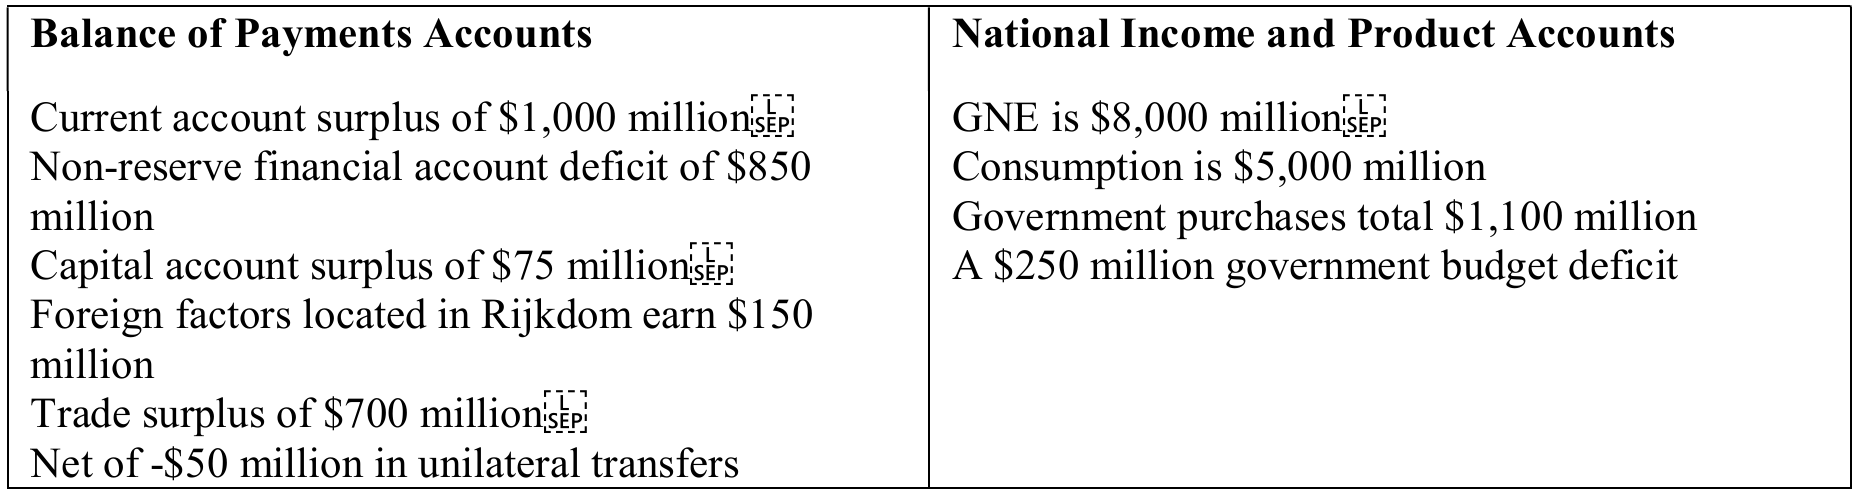
\includegraphics[width=0.95\textwidth]{img/ps01_0103.png}
	%% \caption{}
	%%\label{}
\end{figure}

\begin{enumerate}[label=\emph{\alph*}), topsep = \lineskip, itemsep = \lineskip, partopsep = \lineskip, parsep = \lineskip]
	\item Calculate Rijkdom’s financial account balance. What has happened to Rijkdom’s
  foreign asset position? Explain in detail in terms of Rijkdomian assets and foreign
  assets (owned by Rijkdomians and foreigners).
	\item Calculate the official settlements balance for Rijkdom. Did the Central Bank of
  Rijkdom experience a decrease or an increase in its foreign reserve holdings?
  Explain this in terms of the figure you calculated and what the official settlements
  balance measures \textit{[we won't talk about the Official Settlements Balance; we just calculate the Official Reserve Transactions (ORT)]}.
  \item Calculate net factor income from abroad for Rijkdom. How much did Rijkdomian
  factors abroad earn?
  \item Is Rijkdom a net lender or a net borrower? Explain how you know.
  \item Calculate Rijkdom’s GDP, GNI, and GNDI.
  \item Calculate investment for Rijkdom.
  \item Calculate Rijkdom’s national savings and private savings.
  \item Suppose that valuation effects imply a capital gain of $\$ 220$ million on external wealth. Calculate the change in Rijkdom’ external wealth. Based on these data discuss the three sources of the change in external wealth. Which one appears to be most important in Rijkdom? Explain.
\end{enumerate}

\dotfill


\textit{a)}

$$FA = -(CA + KA) = -(1\,000 + 75) = -1\,075 \rightarrow \text{ net importer of assets}$$

\textit{b)}

$$ORT = FA - FA^{NR} = -1\,070 + 850 = -225 \ (<0) \rightarrow \text{ Central Bank is accumulating foreign reserves}$$

\textit{c)}

$$ NFIA = CA - TB - NUT = 1\,000 - 700 + 50 = 350 $$
$$ X^{FS} = NFIA + M^{FS} = 350 + 150 = 500 $$

\textit{d)}

$$ FA < 0 \rightarrow \text{ net lender} $$

\textbf{e)}

\begin{align*}
   GDP &= A + TB = 8\,000 + 700 = 8\,700 \\
   GNI &= GDP + NFIA = 8\,700 + 350 = 9\,050\\
   GNDI &\overset{1}{=} GNI + NUT = 9\,050 + (-50) = 9\,000\\
   &\overset{2}{=} A + CA = 8\,000+1\,000 = 9\,000
\end{align*}

\textit{f)}

$$ I = A - C - G = 8\,000-5\,000-1\,000 = 1\,900$$

\textit{g)}

\begin{align*}
   S &\overset{1}{=} CA + I = 1\,000 + 1\,900 = 2\,900 \\
   &\overset{2}{=} Y - C - G = 9\,000 - 5\,000 - 1\,000 = 2\,900\\
   S_P &\overset{1}{=} S - S_G = 2\,900 - (-250) = 3\,150\\
   &\overset{2}{=} Y -C-T=Y-C-(G-\textit{ Budget Deficit}) = 9\,000-5\,000 - (1\,100 - 250) = 3\,150
\end{align*}

\textit{h)}

$$\Delta \textit{external wealth} = \textit{valuation effects} + (-FA) =  \textit{capital gains on K} + (CA + KA) = 1\,295$$

The three sources are: (1) cap gains; (2) CA contributions, positive if savings bigger than investments; (3) KA, if people are more generous.

\clearpage

% Question 1.4
\textbf{1.4.}

Explain how each of the following transactions generates two entries – a credit and a debit- in the American balance of payments accounts, and describe how each entry would be classified:

\begin{enumerate}[label=\emph{\alph*}), topsep = \lineskip, itemsep = \lineskip, partopsep = \lineskip, parsep = \lineskip]
	\item A U.S. airplane manufacturer imports $\$600\,000$ in parts from a Canadian firm. It uses a U. S. bank account to pay for the parts.
  \item The Bank of England (U. K. central bank) buys $\$2$ million in U.S. Treasury bonds
  from an American securities firm.
  \item An Italian tourist charges $\$400$ to his Mastercard (issued by an Italian bank) for a
  hotel room in NewYork City.
  \item A Chinese catering company purchases $\$30,000$ in helium tanks from a U. S. welding
  firm. The Chinese catering company uses deposits from a bank in China.
  \item A French firm forgives a $\$250\,000$ loan to an oil refinery located in Louisiana
  following a hurricane.
  \item The United States donates $\$8$ million in medical and food supplies to Lebanon
  following a month-long war.
  \item An American buys a share of German stock, paying the seller with a check on an
  American bank.
  \item An American buys an ink-jet fax machine from the Italian company Olivetti and pays
  for the purchase with a $\$1\,000$ check, which is then deposited at New York Citibank.
  \item An American pays for a dinner in France $\$200$, placing the charge on a Visa credit
  card.
  \item U.S banks forgive $\$5\,000$ in debt owed to them by the government of Bygonia.
  \item A U.S. owned factory in Britain uses local earnings to buy additional machinery.
  \item The Korean government carries out an official foreign exchange intervention in which
  it uses dollars held in an American bank to buy Korean currency from its citizens.
\end{enumerate}

\dotfill

\textit{a)}

\vspace{0.075in}
Therui udohvdopbj
\vspace{0.075in}

\textit{b)}

\vspace{0.075in}
Therui udohvdopbj
\vspace{0.075in}

\textit{c)}

\vspace{0.075in}
Therui udohvdopbj
\vspace{0.075in}

\textit{d)}

\vspace{0.075in}
Therui udohvdopbj
\vspace{0.075in}

\textit{e)}

\vspace{0.075in}
Therui udohvdopbj
\vspace{0.075in}

\textit{f)}

\vspace{0.075in}
Therui udohvdopbj
\vspace{0.075in}

\textit{g)}

\vspace{0.075in}
Therui udohvdopbj
\vspace{0.075in}

\textit{h)}

\vspace{0.075in}
Therui udohvdopbj
\vspace{0.075in}

\textit{i)}

\vspace{0.075in}
Therui udohvdopbj
\vspace{0.075in}

\textit{j)}

\vspace{0.075in}
Therui udohvdopbj
\vspace{0.075in}

\textit{k)}

\vspace{0.075in}
Therui udohvdopbj
\vspace{0.075in}

\textit{l)}

\vspace{0.075in}
Therui udohvdopbj
\vspace{0.3in}

\clearpage

% Question 1.5
\textbf{1.5.}

(Feenstra and Taylor) Consider the economy of Aureus. In Aureus, domestic investment is $\$300$ million and its residents earned $\$10$ million in capital gains during 2006. Residents of Aureus purchased $\$150$ million in new foreign assets during the year and foreigners purchased $\$120$ million in Aureus assets. Assume the valuation effects total $\$1$ million in capital gains. Assume $KA = 0$.

\begin{enumerate}[label=\emph{\alph*}), topsep = \lineskip, itemsep = \lineskip, partopsep = \lineskip, parsep = \lineskip]
	\item Calculate the change in domestic wealth in Aureus.
  \item Calculate the change in external wealth for Aureus.
  \item Calculate the total change in wealth for Aureus.
  \item Calculate domestic savings for Aureus.
  \item Calculate Aureus’ current account. Is the CA in deficit or surplus?
\end{enumerate}

\dotfill

\textit{a)}

$$\Delta \textit{domestic wealth} = I + \textit{capital gains on K} =  300 + 10 = 310$$

\textit{b)}

$$\Delta \textit{external wealth} =\textit{valuation effects} + (-FA) =  1 - (120-150) = 31$$

\textit{c)}

$$\Delta \textit{total wealth} =\Delta \textit{domestic wealth} + \Delta \textit{external wealth} =  310 + 31 = 341$$

\textit{d)}

$$\Delta \textit{total wealth} = S + KA + \textit{capital gains on K} + \textit{capital gains on $(A-L)$} $$
$$ S = 341 - 0 - (10 + 1) =  330$$

\textit{e)}

$$ CA = S - I = 330 - 300 = 30 \ (>0) \rightarrow \text{ surplus}$$

\clearpage

% Question 1.6
\textbf{1.6.}

A hypothetical economy, Endor, was just hit by a hurricane. As a consequence, some information on the national accounts was lost. The following table reports the information that was possible to retrieve from the debris, for the year 2014:

\begin{figure}[!htb]
	\centering
	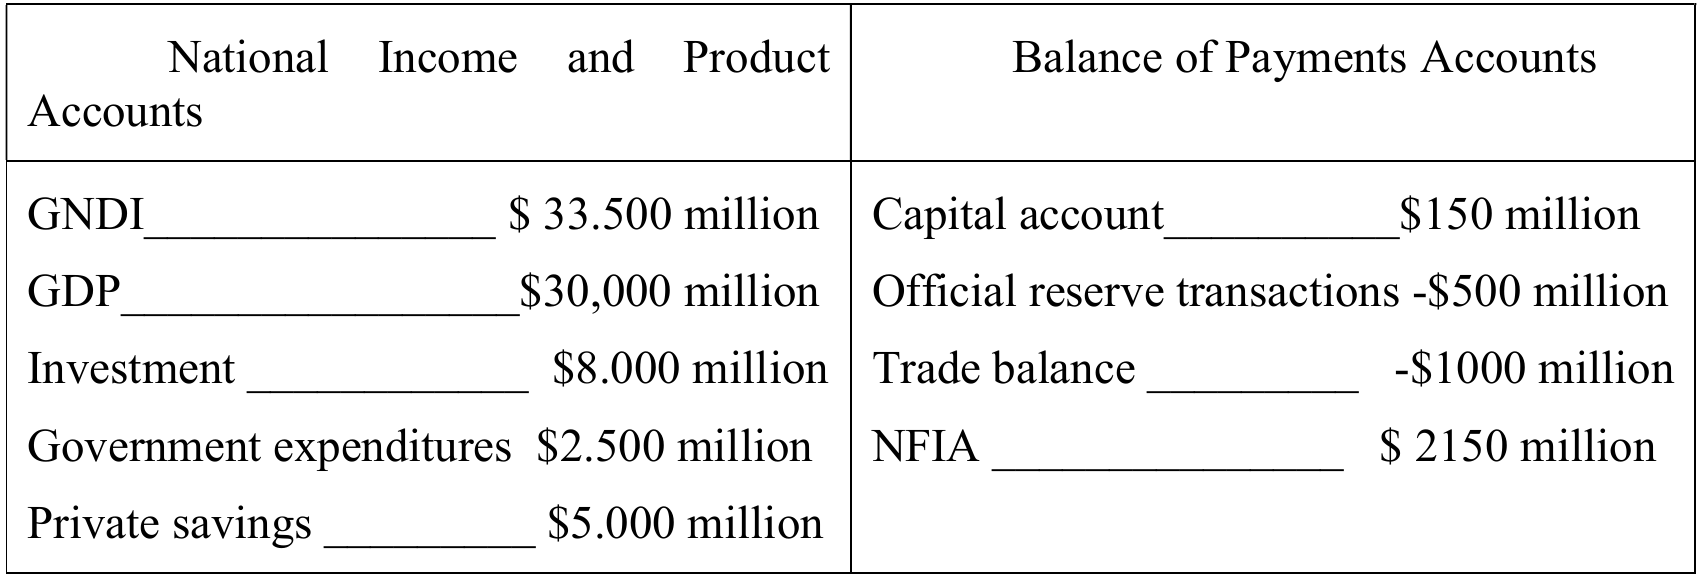
\includegraphics[width=0.95\textwidth]{img/ps01_0106.png}
	%% \caption{}
	%%\label{}
\end{figure}

\begin{enumerate}[label=\emph{\alph*}), topsep = \lineskip, itemsep = \lineskip, partopsep = \lineskip, parsep = \lineskip]
	\item  Calculate Endor’s current account and the financial account balances. Is Endor a net lender or a net borrower? Explain your conclusions.
	\item Compute Endor’s consumption and taxes. Is Endor government running a public
  deficit or surplus?
  \item Calculate the non-reserve financial account balance. Interpret the value of the Offical Reserve Transactions balance and explain what it measures. How can these two balances be related to the Official Settlements balance?
  \item In the aftermath of the hurricane, the two closest Endor’s neighbours prompted to offer help in different ways: the Republic of Naboo has donated $\$20$ million in medical and food supplies and the government of Coruscant has forgiven a $\$5$ million in debt owed to them by the government of Endor.
	\begin{enumerate}[label=\roman*., topsep = \lineskip, itemsep = \lineskip, partopsep = \lineskip, parsep = \lineskip]
		\item Explain how these transactions affected Endor’s balance of payments accounts, describing
    how each entry would be classified.
		\item What will be the effect of this transactions over Endor’s current account balance, GDP, GNDI, and capital account and financial account balances? And over Endor’s net international investment position?
	\end{enumerate}
\end{enumerate}

\dotfill

\textit{a)}


$$CA =  GNDI - GDP + TB = 33\,500  - 30\,000 + (-1\,000) = 2\,500$$
$$FA =  -(CA + KA) = -(2\,500+150) = -2\,350 \rightarrow \text{ net lender}$$


\textit{b)}

$$C =  GDP - I - G - TB = 30\,000 - 8\,000 - 2\,500 - (-1\,000) = 20\,500$$
$$T =  GNDI - S_P - C = 33\,500 - 500 - 2\,650$$
$$S_G = T - G = 8\,000-2\,500 = 5\,500 \rightarrow \text{surplus}$$

\newpage
\textit{c)}

$$ FA^{NR} = FA - ORT = (-2\,650) - (-500) = -2\,150 $$

\textit{d)}

\textit{d)} i.


$$U^{IN} \uparrow \ \rightarrow CA \uparrow$$
$$M \uparrow \ \rightarrow TB \downarrow \ \rightarrow CA  \uparrow$$
$$KA \uparrow, X^A \downarrow \ \rightarrow FA \downarrow$$


\textit{d)} ii.

$$ \Delta GDP = -20$$
$$ \Delta GNDI = 0$$

\clearpage

%%%%%%%%%%%%%%%%%%%%%%%%%%%%%%%%%%%%%%%%%%%%%%%%%%%%%%%%%%%%%%%%%
\textbf{2.1 — (Closed vs Open)}

Consider a two-period endowment economy, where the preferences of the representative consumer are given by $U=\ln{C_1} + 0.8\ln{C_2}$. In this economy, current and future GDP are $Q_1 = 1125$ and $Q_2 = 1350$.

\begin{enumerate}[label=\emph{\alph*}), topsep = \lineskip, itemsep = \lineskip, partopsep = \lineskip, parsep = \lineskip]
	\item Find out the equilibrium interest rate when the economy is closed to capital flows. Comparing to the rate of time preference, is this an expected result?
	\item Suppose that the economy opens to international flows of capital and that the world interest rate is $r^\star = 0.5$. Describe the impact of trade openness in a graph and compute the current and future:
	\begin{enumerate}[label=\roman*., topsep = \lineskip, itemsep = \lineskip, partopsep = \lineskip, parsep = \lineskip]
		\item Consumption
    \item Trade balance
    \item GNI
    \item Current account
    \item Net international investment position
	\end{enumerate}
	\item Departing from $\mathit{b)}$, examine the implications of a fall in the interest rate to $r^\star = 0$. Represent this in a graph. Will the country be better off or worse off?
\end{enumerate}

\dotfill

\textsc{Answer.}

\clearpage
%%%%%%%%%%%%%%%%%%%%%%%%%%%%%%%%%%%%%%%%%%%%%%%%%%%%%%%%%%%%%%%%%
\textbf{2.2 — (Temporary versus permanent income shocks)}

\dotfill

\textsc{Answer.}

\clearpage
%%%%%%%%%%%%%%%%%%%%%%%%%%%%%%%%%%%%%%%%%%%%%%%%%%%%%%%%%%%%%%%%%
\textbf{2.3 — (Infinite Horizon)}

\dotfill

\textsc{Answer.}

\clearpage
%%%%%%%%%%%%%%%%%%%%%%%%%%%%%%%%%%%%%%%%%%%%%%%%%%%%%%%%%%%%%%%%%
\textbf{2.4 — (Small open economy with production)}

\dotfill

\textsc{Answer.}

\clearpage
%%%%%%%%%%%%%%%%%%%%%%%%%%%%%%%%%%%%%%%%%%%%%%%%%%%%%%%%%%%%%%%%%
\textbf{2.5 — (Small economy with production: temporary shock, productivity shock)}

\dotfill

\textsc{Answer.}

\clearpage
%%%%%%%%%%%%%%%%%%%%%%%%%%%%%%%%%%%%%%%%%%%%%%%%%%%%%%%%%%%%%%%%%
\textbf{2.6 — (Small economy with production: productivity shock)}


\dotfill

\textsc{Answer.}

\clearpage
%%%%%%%%%%%%%%%%%%%%%%%%%%%%%%%%%%%%%%%%%%%%%%%%%%%%%%%%%%%%%%%%%
\textbf{2.7 — (Investment, Infinite Horizon)}

\dotfill

\textsc{Answer.}

\clearpage
%%%%%%%%%%%%%%%%%%%%%%%%%%%%%%%%%%%%%%%%%%%%%%%%%%%%%%%%%%%%%%%%%
s

\textsc{Answer.}

\clearpage
%%%%%%%%%%%%%%%%%%%%%%%%%%%%%%%%%%%%%%%%%%%%%%%%%%%%%%%%%%%%%%%%%
\textbf{2.9 — (Risk-diversification)}

\begin{figure}[!htb]
	\centering
	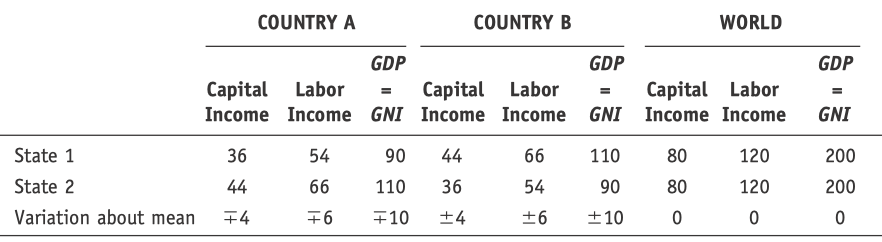
\includegraphics[width=0.95\textwidth]{img/ps02_risk-diversification.png}
	%% \caption{}
	%%\label{}
\end{figure}


\end{document}
